\section{Casi d'uso}
\subsection{Scopo}
Lo scopo di questa sezione è la descrizione in elenco di tutti i casi d'uso individuati dal gruppo, in riferimento alle funzionalità dell'applicazione.
\subsection{Attori}
Come accordato con il proponente, non essendo richiesto alcun servizio di autenticazione attraverso un login o una registrazione, è presente un solo attore che può interagire con l'applicazione web:

\begin{figure}[h]
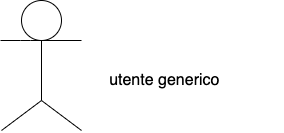
\includegraphics[width=5cm]{section/images/utente.png}
\centering
\caption{Gerarchia attori}
\end{figure}

\begin{description}
\item[Utente generico]:
Si riferisce all'utente utilizzatore che può accedere alla piattaforma.
\end{description}
Per un eventuale gestione di dati in più sessioni è quindi richiesta la funzionalità di poter salvare il proprio lavoro in un file scaricabile, che può poi essere successivamente caricato sulla piattaforma permettendo la ripresa del lavoro.
\subsection{Elenco casi d'uso}
Di seguito sono riportati tutti i casi d'uso che coinvolgono l'utente:
\begin{figure}[h]
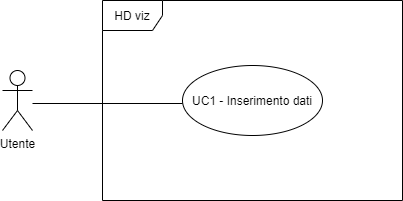
\includegraphics[width=10cm]{section/images/HDviz.png}
\centering
\caption{Casi d'uso dell'utente}
\end{figure}
\subsubsection{UC1 - Inserimento dati}
\begin{figure}[h]
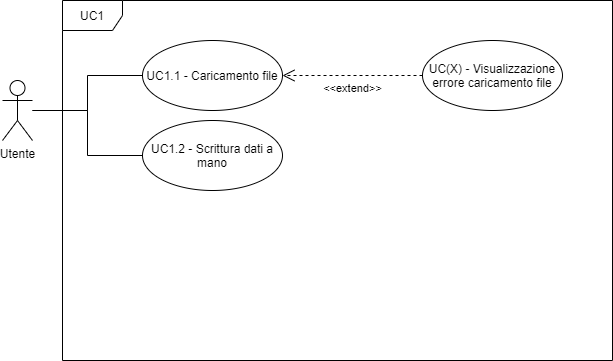
\includegraphics[width=\linewidth]{section/images/UC1-Inserimentodati.png}
\centering
\caption{UC1 - Inserimento dati}
\end{figure}
\begin{itemize}
	\item \textbf{Attore primario}: Utente.
	\item \textbf{Precondizioni}: Il sistema è raggiungibile e funzionante.
	\item \textbf{Postcondizioni}: I dati sono stati inseriti nel database.
	\item \textbf{Scenario principale}:
		\begin{enumerate}
			\item L'utente seleziona "inserisci dati";
			\item L'utente può decidere se:
			\begin{enumerate}
			\item caricare un file contenente dati [UC1.1].
			\item scrivere i dati a mano [UC1.2].
			\end{enumerate}
		\end{enumerate}
	\item \textbf{Estensioni}:
\end{itemize}
\subsubsection{UC1.1 - Caricamento file}
\begin{itemize}
	\item \textbf{Attore primario}: Utente.
	\item \textbf{Precondizioni}: L'utente è in possesso di un file contenente i dati che vuole inserire. L'utente ha selezionato la voce "inserisci dati".
	\item \textbf{Postcondizioni}: Viene visualizzato un messaggio che avvisa l'utente del corretto caricamento del file e della sua validità.
	\item \textbf{Scenario principale}:
	\begin{enumerate}
		\item L'utente seleziona "carica file";
		\item L'utente seleziona il file da caricare;
	\end{enumerate}
	\item \textbf{Estensioni}:
	\begin{enumerate}[(a)]
		\item Nel caso in cui il file abbia un formato sbagliato:
		\begin{enumerate}[1.]
			\item i dati non vengono caricati nel database;
			\item viene visualizzato un errore esplicativo [UCX].
		\end{enumerate}
	\end{enumerate}
\end{itemize}
\subsubsection{UC1.2 - Scrittura dati a mano}

\subsubsection{UCX - Visualizzazione errore caricamento file}